\documentclass{article}

\usepackage{graphicx}
\usepackage{tabularx}
\usepackage{lastpage}
\usepackage{tikz}
\usetikzlibrary{automata}
\usepackage{qtree}

\date{}
\author{Robert Krency}
\title{Project 1}

% Geometry 
\usepackage{geometry}
\geometry{letterpaper, left=20mm, top=20mm, right=20mm, bottom=20mm}

% Fancy Header
\usepackage{fancyhdr}
\fancyhf{}
\lhead{CSC 475}
\rhead{Krency}
\cfoot{Page \thepage \hspace{1pt} of \pageref{LastPage}}

% Add vertical spacing to tables
\renewcommand{\arraystretch}{1.4}

% Document
\begin{document}

\maketitle
\thispagestyle{fancy}

\subsection*{Q1 For each of the following languages, find a grammar that generates it.}

\subsubsection*{$L = \{ a^{n}b^{2n} : n \geq 0 \}$}

\hspace*{1cm}$ G = ( \{S\}, \{a,b\}, S, \{\ S\ \rightarrow\ \lambda\ |\ aSbb\ \} ) $

\subsubsection*{$L = \{ a^{m}b^{n} : m \geq n \geq 0\}$}

\hspace*{1cm}$ G = ( \{ S \}, \{ a,b \}, S, \{\ S\ \rightarrow\ \lambda\ |\ aS\ |\ aSb\ \} ) $


\vspace{5mm}
\subsection*{Q2 Construct an accepting DFA for each of the requirements below:}

\vspace{5mm}

\subsubsection*{All strings on $\{0,1\}$ containing 00 but not 000}

\begin{figure}[h]
    \begin{center}
    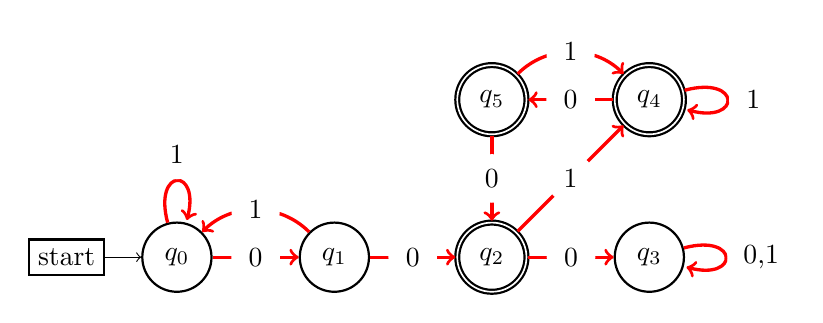
\begin{tikzpicture}
    
        \begin{scope}[every node/.style={circle,thick,draw}]
            \node[initial,state] (1) at (0,0) {$q_0$};
            \node[state] (2) at (2,0) {$q_1$};
            \node[state,accepting] (3) at (4,0) {$q_2$};
            \node[state] (4) at (6,0) {$q_3$};
            \node[state,accepting] (5) at (6,2) {$q_4$};
            \node[state,accepting] (6) at (4,2) {$q_5$};
        \end{scope}
    
        \begin{scope}[every node/.style={fill=white,circle}, every edge/.style={draw=red,very thick}]
            \path [->] (1) edge [loop above] node {1} (1);
            \path [->] (1) edge node {0} (2);
            
            \path [->] (2) edge [out=135, in = 45, looseness=1 ]node {1} (1);
            \path [->] (2) edge node {0} (3);
            
            \path [->] (3) edge node {0} (4);
            \path [->] (3) edge node {1} (5);
            
            \path [->] (4) edge [loop right] node {0,1} (4);
            
            \path [->] (5) edge [loop right] node {1} (5);
            \path [->] (5) edge node {0} (6);
            
            \path [->] (6) edge [out=45, in=135, looseness=1] node {1} (5);
            \path [->] (6) edge node {0} (3);
        \end{scope}
    
    \end{tikzpicture}
    
    \end{center}
\end{figure}

\subsubsection*{All strings on $\{0,1\}$ with the leftmost symbol differing from the rightmost one}

\begin{figure}[h]
    \begin{center}
    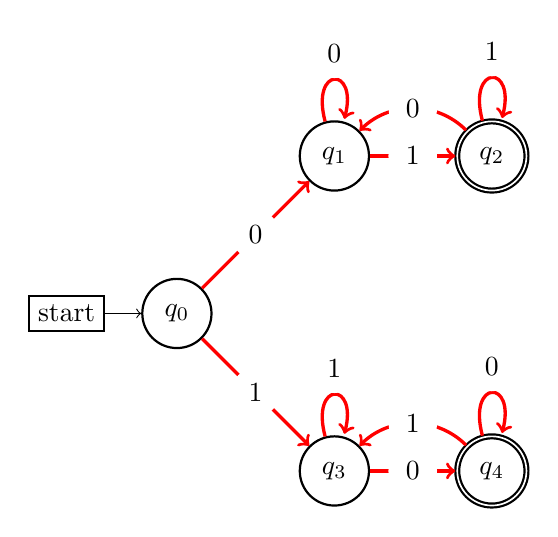
\begin{tikzpicture}
    
        \begin{scope}[every node/.style={circle,thick,draw}]
            \node[initial,state] (1) at (0,0) {$q_0$};
            \node[state] (2) at (2,2) {$q_1$};
            \node[state,accepting] (3) at (4,2) {$q_2$};
            \node[state] (4) at (2,-2) {$q_3$};
            \node[state,accepting] (5) at (4,-2) {$q_4$};
        \end{scope}
    
        \begin{scope}[every node/.style={fill=white,circle}, every edge/.style={draw=red,very thick}]
            \path [->] (1) edge node {0} (2);
            \path [->] (1) edge node {1} (4);

            \path [->] (2) edge node {1} (3);
            \path [->] (2) edge [loop above] node {0} (2);

            \path [->] (3) edge [out=135, in=45, looseness=1] node {0} (2);
            \path [->] (3) edge [loop above] node {1} (3);

            \path [->] (4) edge node {0} (5);
            \path [->] (4) edge [loop above] node {1} (4);

            \path [->] (5) edge [out=135, in=45, looseness=1] node {1} (4);
            \path [->] (5) edge [loop above] node {0} (5);
        \end{scope}
    
    \end{tikzpicture}
    
    \end{center}
\end{figure}

\pagebreak

\subsection*{Q3 Equivalent DFA}

\begin{figure}[h]
    \begin{center}
    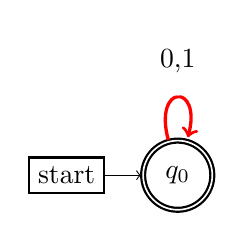
\begin{tikzpicture}
    
        \begin{scope}[every node/.style={circle,thick,draw}]
            \node[initial,state,accepting] (1) at (0,0) {$q_0$};


        \end{scope}
    
        \begin{scope}[every node/.style={fill=white,circle}, every edge/.style={draw=red,very thick}]
            \path [->] (1) edge [loop above] node {0,1} (1);
        \end{scope}
    
    \end{tikzpicture}
    
    \end{center}
\end{figure}


\subsection*{Q4 Prove that language $L = \{ a^n: n \geq 1 \} \cup \{ b^ma^k: m \geq 2, k \geq 0 \} $}

As the following DFA accepts language $L$, it is therefore regular.

\begin{figure}[h]
    \begin{center}
    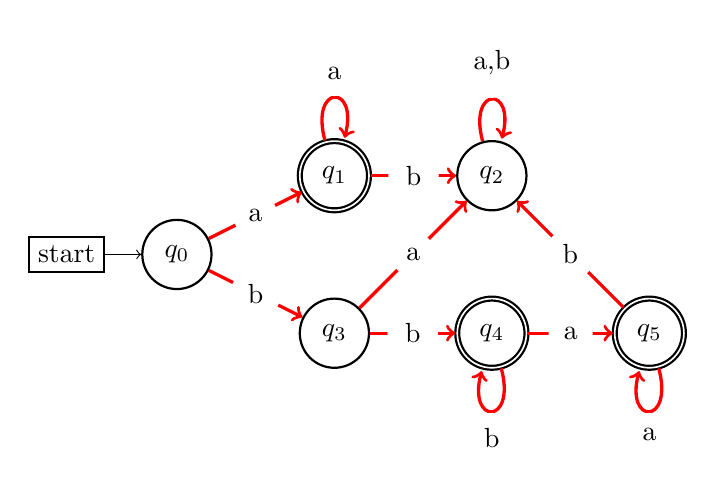
\begin{tikzpicture}
    
        \begin{scope}[every node/.style={circle,thick,draw}]
            \node[initial,state] (1) at (0,0) {$q_0$};
            \node[state,accepting] (2) at (2,1) {$q_1$};
            \node[state] (3) at (4,1) {$q_2$};
            \node[state] (4) at (2,-1) {$q_3$};
            \node[state,accepting] (5) at (4,-1) {$q_4$};
            \node[state,accepting] (6) at (6,-1) {$q_5$};
        \end{scope}
    
        \begin{scope}[every node/.style={fill=white,circle}, every edge/.style={draw=red,very thick}]
            \path [->] (1) edge node {a} (2);
            \path [->] (1) edge node {b} (4);
            
            \path [->] (2) edge [loop above] node {a} (2);
            \path [->] (2) edge node {b} (3);
            
            \path [->] (3) edge [loop above] node {a,b} (2);
            
            \path [->] (4) edge node {a} (3);
            \path [->] (4) edge node {b} (5);
            
            \path [->] (5) edge node {a} (6);
            \path [->] (5) edge [loop below] node {b} (5);
            
            \path [->] (6) edge [loop below] node {a} (6);
            \path [->] (6) edge node {b} (3);
        \end{scope}
    
    \end{tikzpicture}
    
    \end{center}
\end{figure}


\subsection*{Q5}

\subsubsection*{Find a regular expression for the set $\{ a^nb^m : n \geq 3, m$ is even$\}$}
\hspace*{1cm} $aaa\ (a)^*\ (bb)^*$

\vspace*{5mm}
\subsubsection*{Give a regular expression for language on $\Sigma = \{ a,b,c \}$: all strings containing exactly one $a$.}
\hspace*{1cm} $\ (b + c)^*\ a\ (b+c)^* $




\pagebreak

\subsection*{Q2 A DFA with both of the criteria, because I misread the question at first:}

Just thought I'd leave this in because I had already completed it.

\begin{figure}[h]
    \begin{center}
    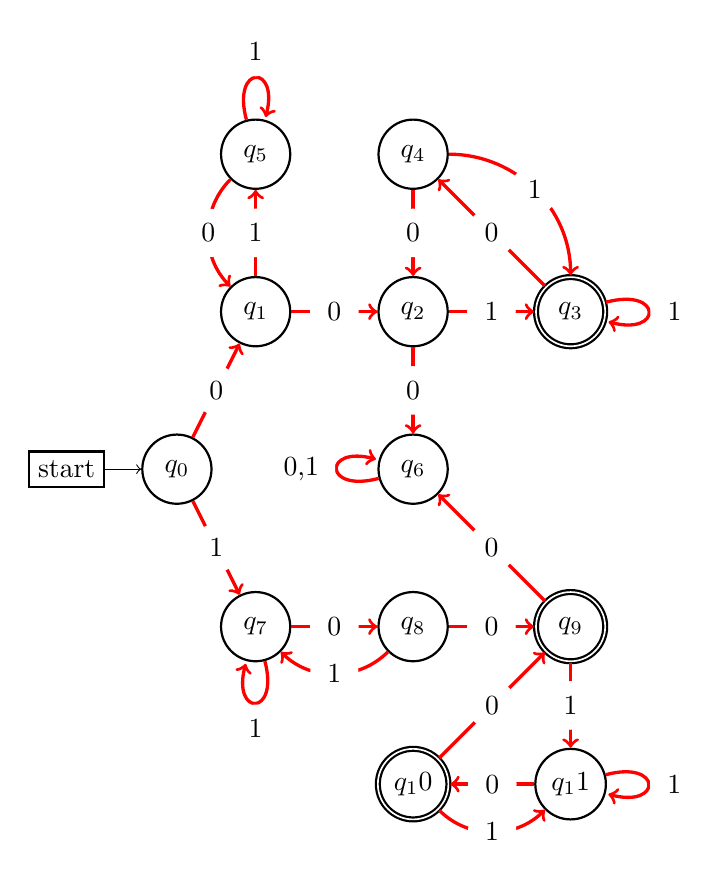
\begin{tikzpicture}
    
        \begin{scope}[every node/.style={circle,thick,draw}]
            \node[initial,state] (1) at (0,0) {$q_0$};

            \node[state] (2) at (1,2)  {$q_1$};
            \node[state] (3) at (3,2)  {$q_2$};
            \node[state,accepting] (4) at (5,2)  {$q_3$};
            \node[state] (5) at (3,4)  {$q_4$};
            \node[state] (6) at (1,4)  {$q_5$};
            \node[state] (7) at (3,0) {$q_6$};

            \node[state] (8) at (1,-2) {$q_7$};
            \node[state] (9) at (3,-2) {$q_8$};
            \node[state,accepting] (10) at (5,-2) {$q_9$};
            \node[state,accepting] (11) at (3,-4) {$q_10$};
            \node[state] (12) at (5,-4) {$q_11$};
        \end{scope}
    
        \begin{scope}[every node/.style={fill=white,circle}, every edge/.style={draw=red,very thick}]
            \path [->] (1) edge node {0} (2);
            \path [->] (1) edge node {1} (8);

            \path [->] (2) edge node {0} (3);
            \path [->] (2) edge [out=90, in=270, looseness=1] node {1} (6);

            \path [->] (3) edge node {1} (4);
            \path [->] (3) edge node {0} (7);

            \path [->] (4) edge node {0} (5);
            \path [->] (4) edge [loop right] node {1} (4);

            \path [->] (5) edge node {0} (3);
            \path [->] (5) edge [out=0, in=90, looseness=1] node {1} (4);

            \path [->] (6) edge [loop above] node {1} (3);
            \path [->] (6) edge [out=225, in=135, looseness=1] node {0} (2);

            \path [->] (7) edge [loop left] node {0,1} (7);

            \path [->] (8) edge [loop below] node {1} (8);
            \path [->] (8) edge node {0} (9);

            \path [->] (9) edge [out=225, in=315, looseness=1] node {1} (8);
            \path [->] (9) edge node {0} (10);

            \path [->] (10) edge node {0} (7);
            \path [->] (10) edge node {1} (12);

            \path [->] (11) edge node {0} (10);
            \path [->] (11) edge [out=315, in=225, looseness=1] node {1} (12);

            \path [->] (12) edge [loop right] node {1} (12);
            \path [->] (12) edge node {0} (11);
            

        \end{scope}
    
    \end{tikzpicture}
    
    \end{center}
\end{figure}


\end{document}